\documentclass{article}

\title{IC internals: replicated state machine}
\subtitle{How the Internet Computer represents and transfers states.}
\date{2021-12-01}
\modified{2025-12-08}

\keyword{ic}

\begin{document}

\epigraph{
My dear, here we must run as fast as we can, just to stay in place.
And if you wish to go anywhere you must run twice as fast as that.
}{
  \href{https://en.wikipedia.org/wiki/Red_Queen_(Through_the_Looking-Glass)}{Red Queen} explaining state sync.
}

\section*

Like all blockchains, the Internet Computer relies on \href{https://en.wikipedia.org/wiki/State_machine_replication}{state machine replication} for fault-tolerance.
This article highlights its two differences from most blockchains:
restricted access to the network state
and support for efficient fault recovery via state checkpoints.

\section{state-machine}{The state machine}

Before we dive into the protocol internals,
let's define its \href{https://en.wikipedia.org/wiki/Finite-state_machine}{state machine}.
The nodes in the protocol are grouped into \emph{subnets}.
Each subnet runs a separate instance of the consensus protocol,
and subnets can exchange messages\sidenote{sn-xnet-protocol}{
  The \nameref{08-ic-xnet} article explains this exchange protocol in more detail.
}.
Consensus orders inputs for the state machine,
which executes \emph{canisters}
(\href{https://webassembly.org/}{WebAssembly} programs).

When formally defined, the state machine has the following components:

\begin{itemize}
\item
  \emph{Inputs} are blocks that contain messages
  destined for canisters hosted on this state machine instance
  and originating from users of canisters on other subnets.
\item
  \emph{Outputs} are
  \emph{state trees} that authenticate the observable state.
\item
  \emph{State} is the data required to serve canisters:
  their WebAssembly modules,
  linear and stable memories, mailboxes,
  and recent execution results.
\item
  \emph{Transition function:}
  Given a new block,
  inject its messages into the canister mailboxes,
  schedule canisters that are ready for execution,
  and record the execution results.
\item
  \emph{Output function} merkelizes the state to produce a state tree.
\item
  The \emph{initial state} is trivial: no canisters, no messages, and no execution results.
\end{itemize}

\section{state-trees}{State trees}

The replica state is a black box,
but for the protocol to be useful,
some pieces of it must be public, including the
results of ingress message execution,
canister metadata (such as Wasm module hashes and certified values),
and messages destined for other subnets.

Accessing the state machine data has two challenges:
\begin{enumerate}
\item
  \emph{Authentication:}
  A client can't trust any single node,
  so nodes must attest their responses.
\item
  \emph{Authorization:}
  Users should only be able to access the data they're authorized to see.
\end{enumerate}

\subsection{stat-auth}{State authentication}

The most straightforward way to authenticate a data structure
is to represent it as a \href{https://en.wikipedia.org/wiki/Merkle_tree}{Merkle tree} over a uniform data format, such as a list or a tree.
The Internet Computer uses \href{https://en.wikipedia.org/wiki/Rose_tree}{rose trees}
with blobs at leaves as its primary data model.
Rose trees are like \textsc{json} objects
that map textual keys to blobs or nested objects:

\begin{code}enum RoseTree {
    Fork(Vec<(String, Box<RoseTree>)>),
    Leaf(Vec<u8>),
}\end{code}

A \emph{state tree} is a merklized rose tree:

\begin{code}enum \b{StateTree} {
    Fork(\b{Hash}, Vec<(\b{Hash}, String, Box<\b{StateTree}>)>),
    Leaf(\b{Hash}, Vec<u8>)
}\end{code}


After each round,
nodes compute the state tree
and exchange their signature shares for its root hash.
The result of this exchange is a threshold signature
that enables a client to authenticate the data received from any node.

\begin{figure}[grayscale-diagram]
  \marginnote{st-structure}{
    A state tree is a labeled merkle tree
    built over the public section of the replica state.
  }
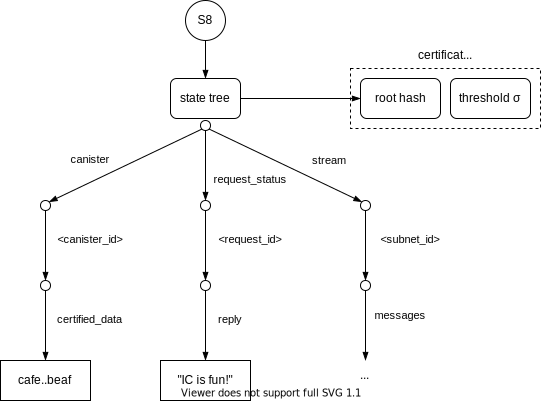
\includegraphics{/images/02-state-tree.svg}
\end{figure}

\subsection{tree-lookup}{Authorization through tree pruning}

A sequence of textual labels identifies a path in a state tree.
Clients access the state by enumerating the paths they're interested in.

Suppose a user sends an ingress message with \textsc{id} \code{1355\ldots 48de}.
The system stores its reply in the state tree at path \code{/request_status/1355\ldots 48de/reply}.
The user connects to a healthy node and calls the \href{https://internetcomputer.org/docs/references/ic-interface-spec#http-read-state}{\code{read_state}} endpoint with that path as an argument.
Upon receiving the request, the node:
\begin{enumerate}
\item
  Fetches the latest certified state tree.
\item
  Checks that the caller has permission to access the path
  (the \code{read_request} signer matches the ingress message signer).
\item
  Trims the state tree to include only the requested path,
  replacing all the pruned branches with their hashes.
\item
  Returns the pruned tree and the state tree certificate.
\end{enumerate}

The resulting tree contains only the data that the caller is authorized to see
and has the same root hash as the original state tree,
so the certificate stays valid.

\begin{figure}[grayscale-diagram]
\marginnote{response-structure}{The logical structure of a tree containing a response to an ingress message.}
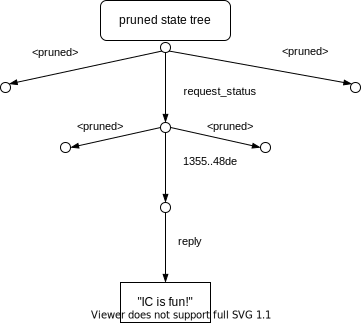
\includegraphics{/images/02-pruned-state-tree.svg}
\end{figure}

The only way for a dishonest node to manipulate the caller
is to reply with an outdated state view,
so honest nodes always include in their output the \code{/time} path that
maps to the timestamp of the block that triggered the tree construction.

\section{state-transfer}{State transfer}

\subsection{checkpoints}{Checkpoints}

When a node crashes,
it loses its in-memory state and must recover before participating again.
To facilitate recovery,
nodes periodically write \emph{checkpoints}---serialized states---to disk.
If a node was offline briefly,
it catches up by replaying blocks from the last checkpoint.
If it was offline longer,
replaying blocks alone would take too long,
so fetching the latest checkpoint from a peer
becomes a more efficient strategy.
The same approach applies when a fresh node joins a subnet.

Most blockchains treat checkpoints as implementation details
and distribute them via a side channel.
In the Internet Computer, state sync is part of the core protocol,
streamlining node operations.

\begin{figure}[grayscale-diagram]
\marginnote{sm-components}{
  State machine components: blocks, states, state trees, and checkpoints.
}
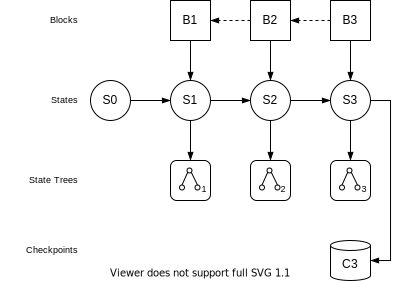
\includegraphics{/images/02-states.svg}
\end{figure}

\subsection{state-artifact}{State as an artifact}

Replicas in a subnet communicate by exchanging \emph{artifacts}
(ingress messages, blocks, random beacons, state certificates)
over a \href{https://en.wikipedia.org/wiki/Peer-to-peer}{peer-to-peer protocol}.
Most artifacts are a few megabytes,
but the protocol can fetch arbitrarily large blobs by slicing them into chunks.
State sync uses this machinery to transfer checkpoints.

The peer-to-peer protocol combines a \href{https://en.wikipedia.org/wiki/Push_technology}{push model} for metadata and a \href{https://en.wikipedia.org/wiki/Pull_technology}{pull model} for data:
Nodes advertise their artifacts
and serve them to interested peers.

Before advertising a checkpoint, a replica computes its \emph{manifest}---%
a summary of the checkpoint directory,
similar to the \code{info} section of a \href{https://en.wikipedia.org/wiki/Torrent_file}{\code{.torrent} file}.
A manifest consists of two tables:
the file table contains file metadata,
the chunk table describes the file contents.

\begin{figure}
\marginnote{mn-manifest-example}{
  A checkpoint manifest example.
  It consists of two tables:
  the file contains file metadata,
  the chunk table describes the contents of these files.
}
\begin{tabular}{rlrl}
  File & Path & Size & Hash \\
  \hrule
0 & \code{canisters/\ldots/queues.pb} & 100 & \code{e3b0c44298fc1c149afbf4c8996fb92427ae41e4649b934c\ldots} \\
1 & \code{canisters/\ldots/memory.bin} & 2101248 & \code{07123e1f482356c415f684407a3b8723e10b2cbbc0b8fcd6\ldots} \\
\end{tabular}
\newline
\newline
\begin{tabular}{rrrrl}
Chunk & File & Offset & Size & Hash \\
\hrule
0 & 0 & 0 & 100 & \code{ad57366865126e55649ecb23ae1d48887544976efea46a48\ldots} \\
1 & 1 & 0 & 1048576 & \code{5feceb66ffc86f38d952786c6d696c79c2dbc239dd4e91b4\ldots} \\
2 & 1 & 1048576 & 1048576 & \code{6b86b273ff34fce19d6b804eff5a3f5747ada4eaa22f1d49\ldots} \\
3 & 1 & 2097152 & 4096 & \code{d4735e3a265e16eee03f59718b9b5d03019c07d8b6c51f90\ldots} \\
\end{tabular}

\end{figure}

Replicas use manifests as blueprints for organizing the data on disk
and for validating the chunks they receive.
A manifest hash identifies the checkpoint as a network artifact.

\begin{figure}[grayscale-diagram]
\marginnote{checkpoint-advert}{A replica advertising a checkpoint as an artifact.}
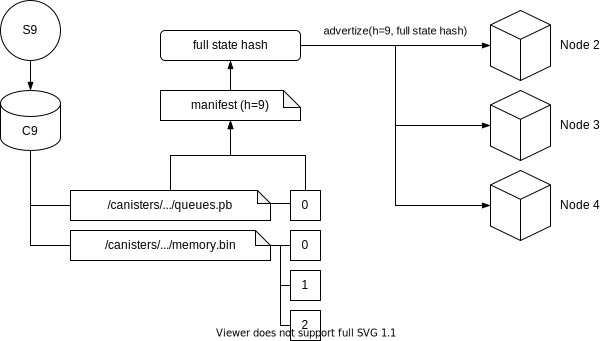
\includegraphics{images/02-checkpoint-artifact.svg}
\end{figure}

\subsection{trigger-transfer}{Triggering state transfer}

The signal that a replica is behind comes from the consensus module.
After every checkpoint, it creates a \emph{catch-up package}---the bill of materials a replica needs to participate in the protocol,
including the \href{https://en.wikipedia.org/wiki/Distributed_key_generation}{\textsc{dkg}} summary, the random beacon value,
and the checkpoint hash.

Suppose a replica crashes after processing nine blocks
and comes back when the network moved on to state 100,
which happened to be the next scheduled checkpoint.
Here is how replica components interact to trigger the state transfer:

\begin{enumerate}
\item
  Consensus observes a catch-up package advertisement and fetches its content.
  The package indicates that the latest recoverable state is 100
  and the its manifest hash is $H_{100}$.
\item
  Consensus checks the latest locally available state height (it's nine).
\item
  Consensus decides that replaying blocks is not an option
  and instructs the State Machine to fetch state 100 with root hash $H_{100}$.
\item
  State Machine subscribes to artifact advertisements
  and initiates the fetch once a matching one arrives.
\end{enumerate}

\subsection{incremental-sync}{Fetching states incrementally}

Once the state machine knows which state it needs to fetch,
it doesn't need any instructions from the consensus module;
it uses the transport module directly.
Continuing our example,
here is how State Machine syncs from state 9 to state 100:

\begin{enumerate}
\item
  Transport delivers an advertisement for a checkpoint with hash $H_{100}$.
  State Machine initiates an artifact fetch.
\item
  State Machine fetches the zeroth chunk, which by convention contains the manifest,
  decodes it,
  and ensures that its hash matches $H_100$.
\item
  State Machine compares the manifests of checkpoint 9 and 100,
  classifying chunks as either \emph{locally available} or \emph{missing.}
\item 
  It copies locally available chunks into their proper positions.
\item
  It instructs Transport to fetch all the missing chunks.
  Transport can stream data from several peers concurrently.
\item
  As Transport delivers chunks,
  State Machine validates their hashes against the manifest
  and puts them into their slots on disk.
\end{enumerate}

When there are no more chunks to fetch,
the checkpoint 100 is finalized.

\begin{figure}[grayscale-diagram]
\marginnote{checkpoint-construct}{A replica constructing a fresh checkpoint by re-using existing chunks and fetching the missing ones.}
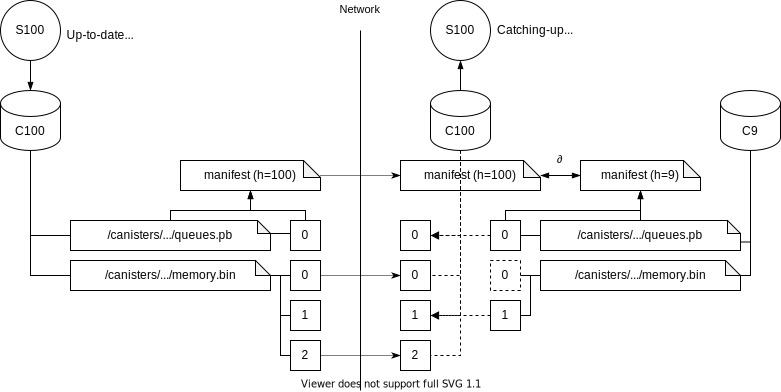
\includegraphics{/images/02-state-sync.svg}
\end{figure}

The state transfer procedure is \emph{incremental:}
A replica that was offline for a brief period fetches only the changed data.
It's also \emph{resumable:}
If a checkpoint goes away before the transfer completes,
the receiver can reuse the fetched chunks in the next sync attempt.

\subsection{state-sync-alternatives}{Paths not taken}

It's instructive to mention alternative rejected state sync protocols.

One early idea involved a catching-up node connecting to a healthy one,
sending its state height,
and receiving all the subsequent state updates.
This protocol has major flaws:
\begin{enumerate}
\item
  It requires versioning every bit of the replica state
  and peppering all state transitions with version updates.
  Missing an update is a nasty bug.
\item
  It pushes most of the work to the healthy node,
  slowing down the subnet.
  A catching-up node has no other useful work,
  so it should bear most costs.
\item
  It's sequential: 
  there is no obvious way to involve more than one sender.
\item
  It isn't resumable:
  If the transfer interrupts,
  the receiver starts from scratch.
\end{enumerate}

Another alternative was to represent the entire replica state as a state tree
and sync these logical trees instead of concrete file system representations.
This approach would make it easier to specify the protocol
and support syncing between \href{https://en.wikipedia.org/wiki/N-version_programming}{replicas written in different languages},
but the extra complexity outweighed the benefits.

\section{conclusion}{Conclusion}

This article focused on two features that differentiate the Internet Computer
from most other blockchains:
\href{#state-tree}{state trees}
and a built-in \href{#state-transfer}{state sync protocol}.
State trees allow clients to query a certified subnet state by talking to a single node.
The state sync protocol allows for fast node recovery and painless reconfiguration.

\end{document}

